
\begin{longtable} { | c | p{12cm} | c | } 
\hline
	ID 	&	Issues	&		 Es. hours \\\hline
	26	& 	Change all buttons	&	8 hours	\\\hline
	27	& 	Change GUI of Viewgroups	&	16 hours	\\\hline
\caption{Issues ID 26 and 27}
\label{tab:spr2_GUIchange}
\end{longtable}

One of the biggest changes from sprint 1 is the entire UI is fitted to match the entire application. This means changing every single button and grid to the templates the GUI group provided. As there is a lot of GUI to change, we have chosen to just describe two examples. The first example of the completely customizable dialog box is shown in listing \ref{lst:GDialog} and shown in figure \ref{fig:GDialog}. We use this several times throughout the application, we use it when editing sequences as a guardian. The example shown is when the guardian tries to exit editing a sequence without having saved. Each button is linked to a XML file determining where the button is displayed in the layout as well as what the headline and description says.

\begin{lstlisting} [caption={Customizable Dialogbox}, label={lst:GDialog}]

    public class backDialog extends GDialog {

        public backDialog(Context context) {

            super(context);

            this.SetView(LayoutInflater.from(this.getContext()).inflate(R.layout.exit_sequence_dialog,null));

            GButton saveChanges = (GButton) findViewById(R.id.save_changes);
            GButton discardChanges = (GButton) findViewById(R.id.discard_changes);
            GButton returntoEditting = (GButton) findViewById(R.id.return_to_editing);


            saveChanges.setOnClickListener(new GButton.OnClickListener() {

                @Override
                public void onClick(View v) {
                    SequenceActivity.this.saveChanges();
                }
            });

            discardChanges.setOnClickListener(new GButton.OnClickListener() {

                @Override
                public void onClick(View v) {
                    finish();
                }
            });

            returntoEditting.setOnClickListener(new GButton.OnClickListener() {

                @Override
                public void onClick(View v) {
                    dismiss();
                }
            });
        }

    }
\end{lstlisting}

\begin{figure} [h!]
\centering
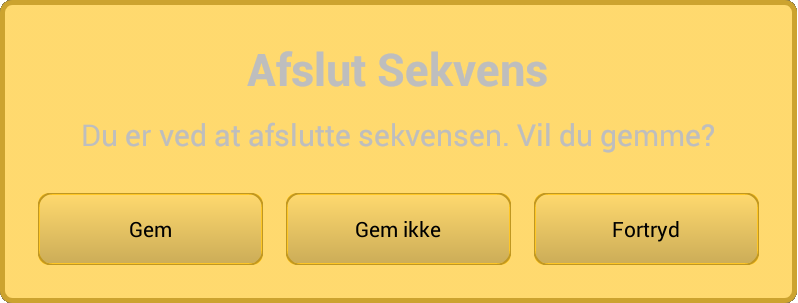
\includegraphics[width=0.65\textwidth]{Pics/Sprint2/dialogs/afslutSekvens.png}
\caption{This dialog box is the result of the code in the listing above}
\label{fig:GDialog}
\end{figure}

The GUI group also provided a list of simple templates e.g. a 2 button dialogmessage. The example shown in \ref{lst:GDialogmessage} is the delete button shown in the overview. The constructor needs the context, an image, a headlline, a description and a functionality for one of the buttons. The second button added in the dialog box is a button that closes the dialog box and returns to the previous state.

\begin{lstlisting}  [caption={GDialogmessage}, label={lst:GDialogmessage}]

    public void deleteSequenceDialog (View v) {
        GDialogMessage deleteSequence = new GDialogMessage(v.getContext(),
            R.drawable.ic_launcher,
            "Slet Sekvens",
            "Du er ved at slette sekvensen, er du sikker paa du vil det?",
            new View.OnClickListener() {
                @Override
                public void onClick(View v) {
			deleteSequence();
                }
            });

\end{lstlisting}

The GComponents group also provided an easy implementation of the buttons. They provided an extension, \ct{GButton} of the android standard \ct{Button}. The implementation was simply refactoring every button to be an instance of GButton instead of Button. A couple of examples are shown in figure \ref{fig:buttons}. In the same vein they provided \ct{GGridView} as an extension to the android standard \ct{GridView}, and example of this is show in \ref{fig:GGridView}.

\begin{figure} [h!]
\centering
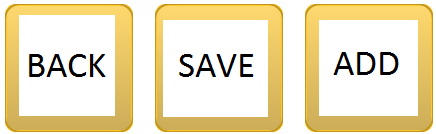
\includegraphics[width=0.5\textwidth]{Pics/Sprint2/dialogs/backSaveAdd.png}
\caption{This is an example of 3 new buttons without final icons}
\label{fig:buttons}
\end{figure}

\begin{figure} [h!]
\centering
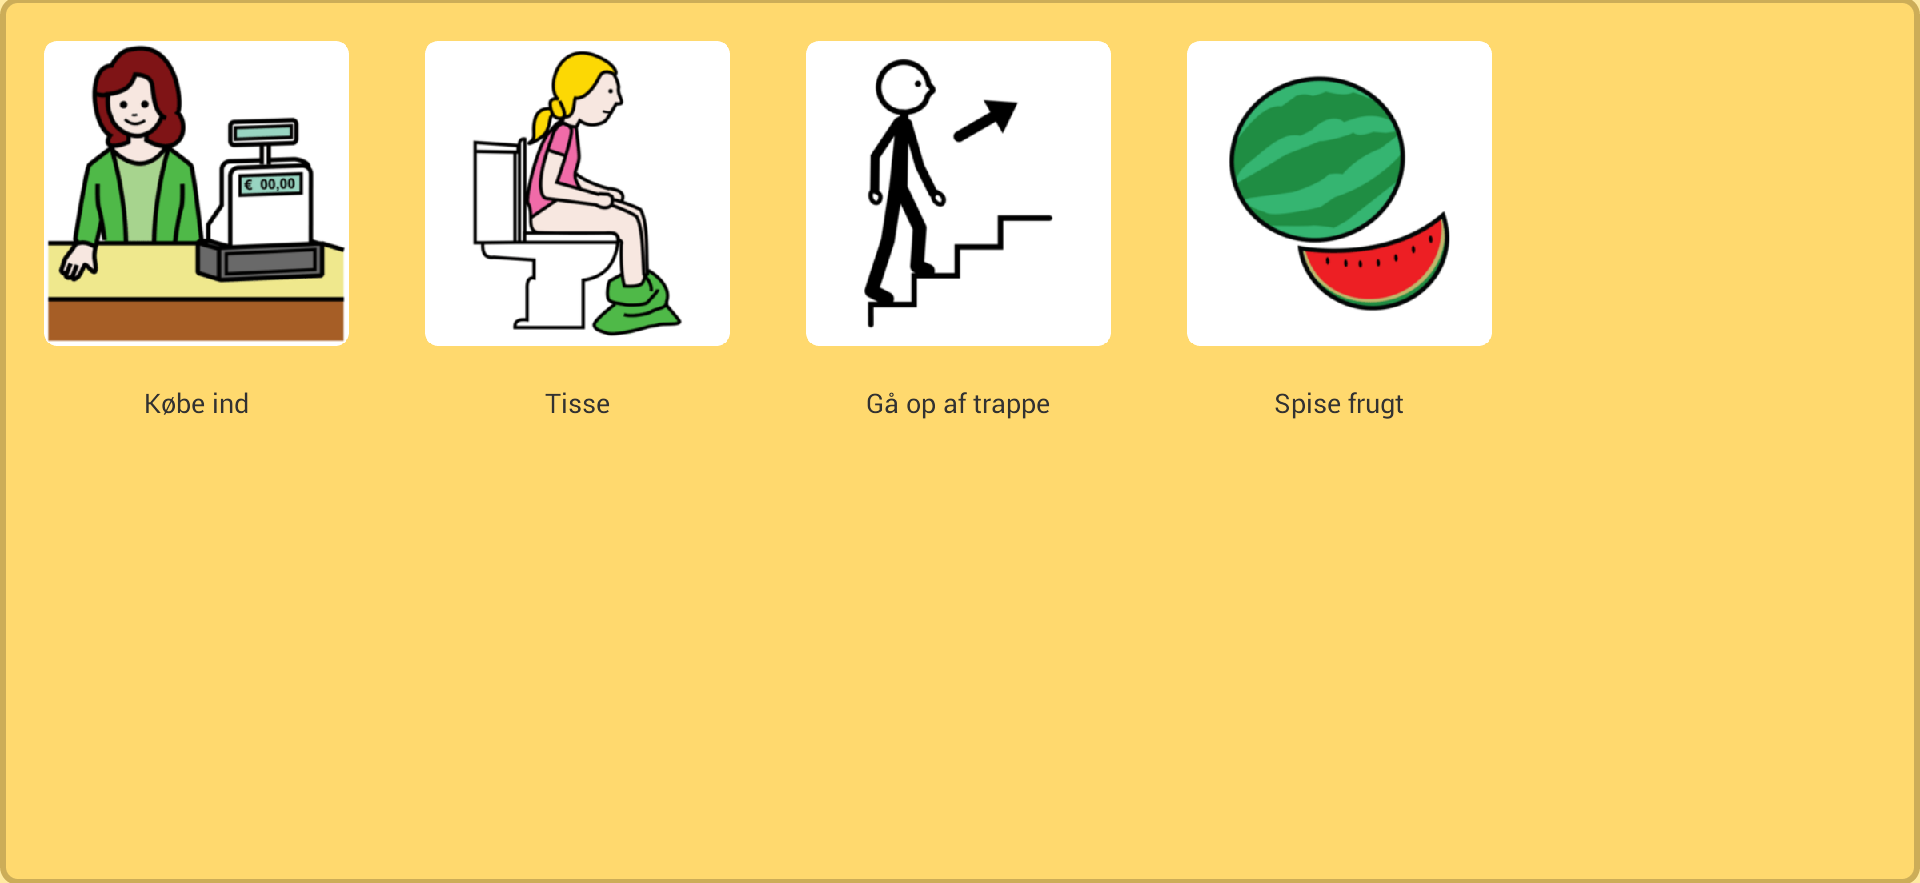
\includegraphics[width=0.9\textwidth]{Pics/Sprint2/dialogs/magicGrid.png}
\caption{This is the grid in mainActivity of a child with 4 different sequences attached}
\label{fig:GGridView}
\end{figure}




